% {{{1 PRELUDE
\documentclass{beamer}

\usepackage[francais]{babel}
% \usepackage[english]{babel}
\usepackage[utf8]{inputenc}
\usepackage[T1]{fontenc}

\usetheme{Frankfurt}

\AtBeginSection[]
{
    \begin{frame}
        \frametitle{Sommaire}
        \tableofcontents[currentsection, hideothersubsections]
    \end{frame}
}

\title[Lissage adaptatif de nuage de points]{Lissage adaptatif de nuage de
    points}
\author[MEYRON Jocelyn]{MEYRON Jocelyn\\\scriptsize{Encadré par:\\ATTALI Dominique\\MÉRIGOT
    Quentin}}
\institute{GIPSA-lab}
\date{\today}

\begin{document}

\begin{frame}
    \titlepage
\end{frame}

\begin{frame}
    \tableofcontents
\end{frame}

% {{{1 INTRODUCTION
\section{Introduction}

\begin{frame}
    \frametitle{Introduction}
    % \framesubtitle{Flot de courbure moyenne}

    Flot de courbure moyenne:
    \begin{itemize}
        \item Faire évoluer une surface en bougeant chaque point: dans la
            direction de la normale et d'une quantité égale à la courbure
            moyenne en ce point
        \item Propriétés lissantes
    \end{itemize}

    \begin{figure}
        \centering
        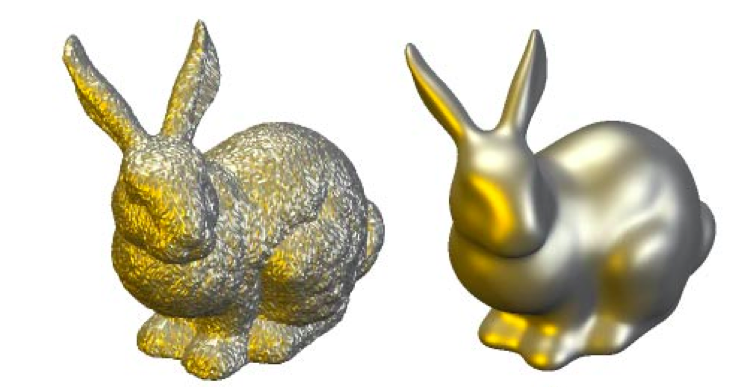
\includegraphics[scale=0.27]{img/mean-curvature-flow-rabbit}
        \caption{Flot de courbure moyenne sur une surface bruitée}
    \end{figure}
\end{frame}

\begin{frame}
    \frametitle{Introduction}
    % \framesubtitle{Objectifs}

    \emph{Objectifs}
    \begin{enumerate}
        \item Flot de courbure moyenne sur des nuages de points: calculer une
            fonctionnelle de l'union des boules (aire, périmètre du bord) et
            faire une descente de gradient
        \item Flot de courbure moyenne anisotrope: remplacer l'union des boules
            par la somme de Minkowski avec un polyèdre convexe
    \end{enumerate}

    \emph{Applications:}
    \begin{enumerate}
        \item Débruitage
        \item Simulation de croissance de cristaux
    \end{enumerate}
\end{frame}

\begin{frame}
    \frametitle{Introduction}
    % \framesubtitle{Quelques notions}

    \begin{definition}[Offset d'un nuage de points]
        Le $r$-offset d'une nuage de points $ P \subseteq \mathbb{R}^d $ est
        défini par:
        $$ P^r = \bigcup_{p \in P} B(p, r) $$
    \end{definition}

    \begin{definition}[$\epsilon$-échantillon]
        Pour une hypersurface $ S $, on dit que $ P \subseteq \mathbb{R}^d $ est
        un $\epsilon$-échantillon de $ S $ si:
        $$ \bigcup_{p \in P} B(p, \epsilon) \subseteq S $$
    \end{definition}
\end{frame}

\begin{frame}[allowframebreaks]
    \frametitle{Introduction}
    % \framesubtitle{Résultats théoriques}

    \begin{theorem}[Approximation de l'aire d'une hypersurface]
        Soit une hypersurface $ S $ de $ \mathbb{R}^d $ et $ P $ un
        $\epsilon$-échantillon de $ S $, alors:
        $$ | \frac{Vol^d(P^r)}{2r} - Vol^{d-1}(S) | \leq \frac{\epsilon^2}{2r^2} +
        O(\frac{\epsilon^4}{r^3}) + O(r^2) $$
    \end{theorem}

    \begin{theorem}[Gradient de l'aire]
        Si $ A = Vol^d(P^r) $ alors en notant $ \nabla_{p_i} A $ la limite
        suivante:
        $$ \lim\limits_{\epsilon \to 0} \frac{A(p_1, \ldots, p_{i-1}, p_i + \epsilon
            \delta p_i, p_{i+1}, \ldots, p_N) - A(p_1, \ldots, p_N)}{\epsilon} $$
        On a:
        $$ \nabla_{p_i} A = \int_{B} \frac{x - p_i}{||x - p_i||} dx $$
        où $ B = \partial B(p_i, r) \cap V(p_i, P) $.
    \end{theorem}

    \begin{theorem}[Approximation de la courbure moyenne]
        Soit une hypersurface $ S $ de $ \mathbb{R}^d $ et soit $ P $ un
        $\epsilon$-échantillon de $ S $, on a:
        $$ \nabla_p A \approx 2 r \vec{\kappa}(p) Vol(V(p, P) \cap
        M) $$
    \end{theorem}
\end{frame}

% {{{1 2D
\section{Cas 2D}

\subsection{Problème}
\begin{frame}
    \frametitle{Problème}
    % \framesubtitle{Flot de courbure moyenne}

    Flot de courbure moyenne sur des nuages de points: descente de gradient
    \begin{itemize}
        \item Calcul du volume (ou du périmètre du bord) de l'union de boules
        \item Calcul du gradient
        \item Déplacement des points (Euler explicite): $ p'_i = p_i - \tau \nabla f (p_i) $ où $
            \tau $ est une constante
    \end{itemize}

    \begin{figure}
        \centering
        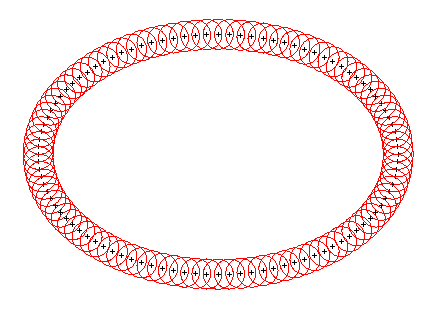
\includegraphics[scale=0.28]{img/ellipse-balls-15}
        \caption{Union de boules autour d'une ellipse}
    \end{figure}
\end{frame}

\begin{frame}
    \frametitle{Problème}
    % \framesubtitle{Outils}

    Outils:
    \begin{itemize}
        \item CGAL: bibliothèque C++ de géométrie algorithmique
        \item Différentiation automatique: calcul de dérivées de fonctions (au
            sens informatique du terme) en surchargeant le type de nombre,
            remplacement de $ x $ par $ x + y\epsilon $ avec $ \epsilon^2 = 0 $
        \item Qt
    \end{itemize}
\end{frame}

\subsection{Estimation de courbure moyenne}
\begin{frame}
    % TODO: ajout erreur
    \frametitle{Estimation de courbure moyenne}
    % \framesubtitle{Exemples}

    Exemples: courbure d'une ellipse
    \begin{figure}
        \centering
        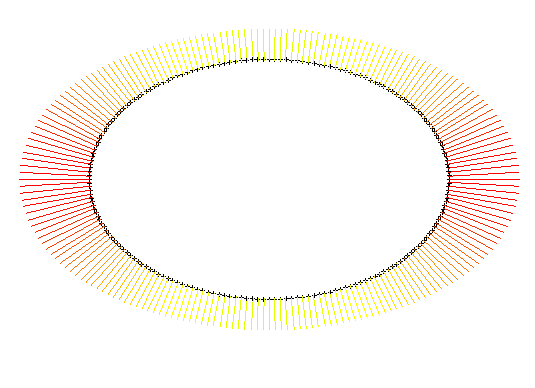
\includegraphics[scale=0.3]{img/curvature-ellipse-200-15-area}
        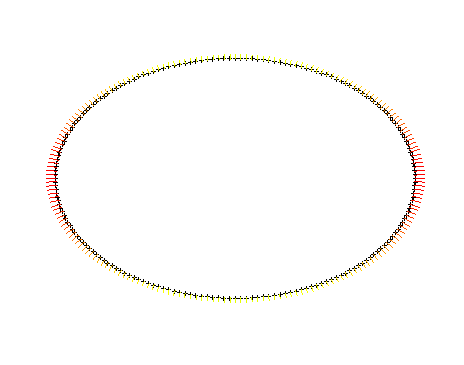
\includegraphics[scale=0.3]{img/curvature-ellipse-200-15-perimeter}
        \caption{Aire / périmètre du bord}
    \end{figure}
\end{frame}

\subsection{Flot de courbure moyenne}
\begin{frame}
    % TODO: meilleures images
    \frametitle{Flot de courbure moyenne}
    % \framesubtitle{Exemples}

    Exemples: flot d'une ellipse
    \begin{figure}
        \centering
        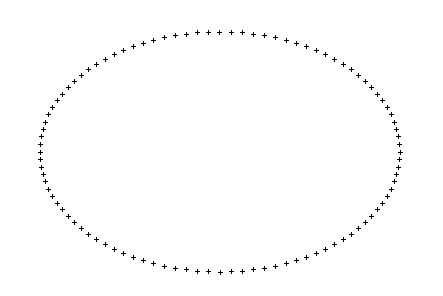
\includegraphics[scale=0.3]{img/ellipse-100-01-15}
        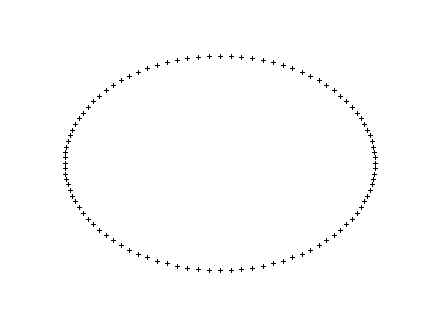
\includegraphics[scale=0.3]{img/ellipse-100-01-15-100}
        \caption{0 / 100 itérations}
    \end{figure}
\end{frame}

% {{{1 3D
\section{Cas 3D}

\subsection{Problème}
\begin{frame}
    \frametitle{Problème}
    % \framesubtitle{Flot anisotrope}

    Flot anisotrope:
    \begin{itemize}
        \item Somme de Minkowski avec un polyèdre convexe
        \item Directions privilégiées
    \end{itemize}

    Différentes méthodes:
    \begin{itemize}
        \item Naïve (approchée)
        \item Formules d'inclusion-exclusion (approchée)
        \item Arrangements 3D (exacte?)
    \end{itemize}
\end{frame}

\subsection{Exemples}
\begin{frame}
    \frametitle{Exemples}
    % \framesubtitle{Polyèdres}

    Polyèdres:
    \begin{itemize}
        \item Discrétisation d'une sphère: estimation de normales
        \item Cube (Norme $ L_{\infty} $)
        \item Bipyramide (Norme $ L_1 $)
    \end{itemize}
\end{frame}

\subsection{Flot}
\begin{frame}
    \frametitle{Estimation de normales}
    % \framesubtitle{Exemples}

    Exemples:
    \begin{figure}
        \centering
        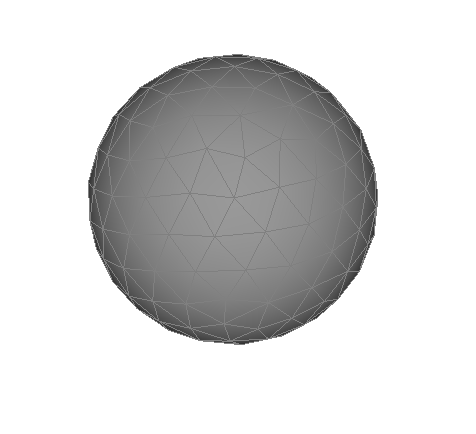
\includegraphics[scale=0.22]{img/sphere-polyhedron-200}
        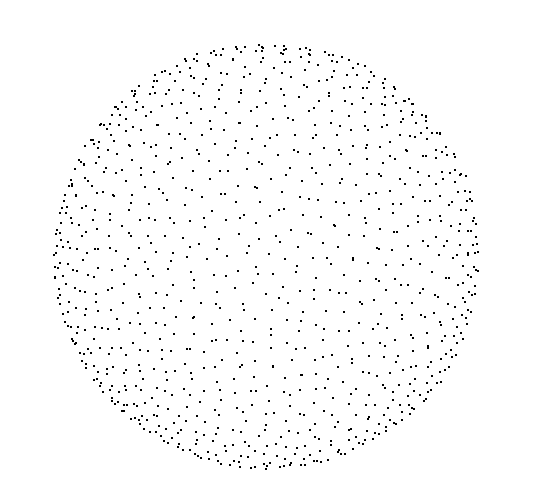
\includegraphics[scale=0.2]{img/sphere-1000}
        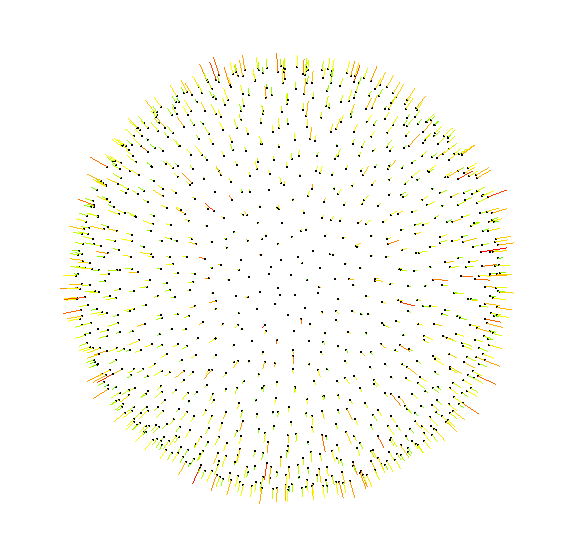
\includegraphics[scale=0.2]{img/sphere-sphere-1000-05}
        \caption{Estimation de normales sur une sphère}
    \end{figure}
\end{frame}

\begin{frame}[allowframebreaks]
    \frametitle{Flot anisotrope}
    % \framesubtitle{Exemples}

    Exemples:
    \begin{figure}
        \centering
        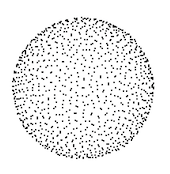
\includegraphics[scale=0.4]{img/sphere-cube-0}
        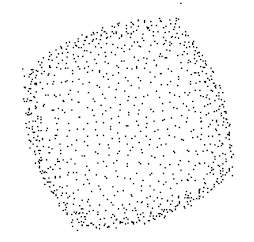
\includegraphics[scale=0.3]{img/sphere-cube-10}
        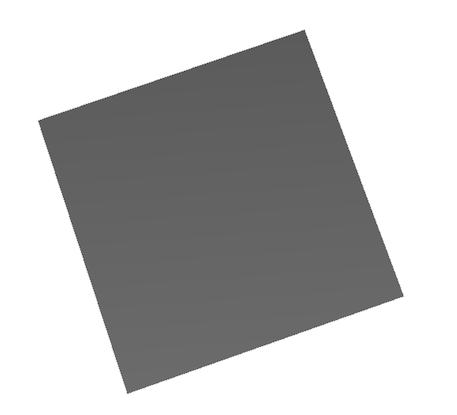
\includegraphics[scale=0.2]{img/sphere-cube-cube}
        \caption{10 itération d'un flot avec un cube}
    \end{figure}

    \begin{figure}
        \centering
        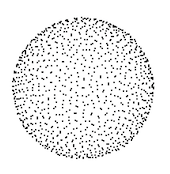
\includegraphics[scale=0.4]{img/sphere-cube-0}
        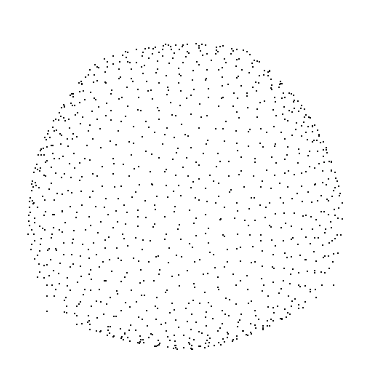
\includegraphics[scale=0.2]{img/sphere-bipyramid-10}
        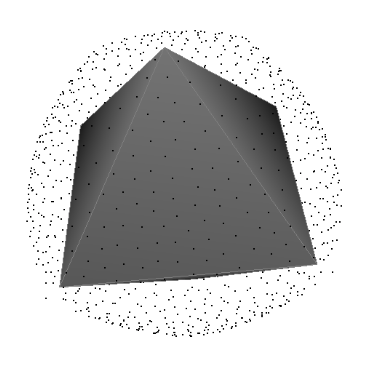
\includegraphics[scale=0.2]{img/sphere-bipyramid-bipyramid}
        \caption{10 itération d'un flot avec une bipyramide}
    \end{figure}
\end{frame}

% {{{1 PERSPECTIVES
\section{Perspectives}

\begin{frame}
    \frametitle{Perspectives}
    % \framesubtitle{Sous-titre}

    \begin{itemize}
        \item Preuve que gradient de l'aire du bord converge vers la courbure
            moyenne
        \item Améliorer calcul en 3D (utilisation d'arrangements 3D)
        \item Mieux comprendre gradient du flot anisotrope
    \end{itemize}
\end{frame}

% \plain{Merci!}

\end{document}

% vim: set spelllang=fr :
